\label{ch:experiment}
Celem doświadczenia jest sprawdzenie, z~jaką dokładnością pojazd jest w~stanie docierać do wartości zadanej, innymi słowy jak bardzo zmniejszyć uchyb, utrzymując jednocześnie zsynchronizowane położenie silników. W tym celu zostaną podjęte następujące kroki:

\begin{enumerate}
    \item Doświadczalne wyznaczenie charakterystyki statycznej
    \item Strojenie równoległe regulatorów PID sygnałów niezależnych silnika prowadzącego i~śledzącego przy 50\%~prędkości i~1.5~m odległości
    \item Strojenie regulatora PID sygnału zależnego silnika śledzącego przy 50\%~prędkości i~1.5~m odległości
    \item Przeprowadzenie pomiarów dla 30\%, 65\% i~100\% prędkości dla 1~m, 1.5~m i~2~m
\end{enumerate}

\section{Charakterystyka statyczna}
Została wyznaczona poprzez wysterowanie silników do stanu semi-ustalonego (ze względu na pewne drobne oscylacje), i~wyciągnięcie średniej z~15 pomiarów. Operację tę powtórzono dla obu silników, dla prędkości od 0\%~do 100\%,~ze skokiem~5\%. Wyznaczona została dla biegu jałowego. Charakterystyka statyczna widoczna jest na Rysunku~\ref{fig:charstatjalowy}. Można zauważyć, że dopiero gdzieś w~przedziale 5\%--10\% mocy, silniki pokonują opór statyczny i~zaczynają się obracać. Poza drobnymi odchyłkami wynikającymi z~niskiej jakości wykonania silników, oraz samej ich natury fizycznej, ich charakterystyki statyczne są w~przybliżeniu liniowe. Widać również, że nawet na biegu jałowym i~bez ograniczeń w~oprogramowaniu, prawy silnik jest o~kilka procent wolniejszy od lewego. Dokładnie to zjawisko, spowodowane m.in. drobnymi różnicami w~budowie fizycznej, postawiono za cel wyeliminować używając enkoderów i~regulatorów PID.

\begin{center}
    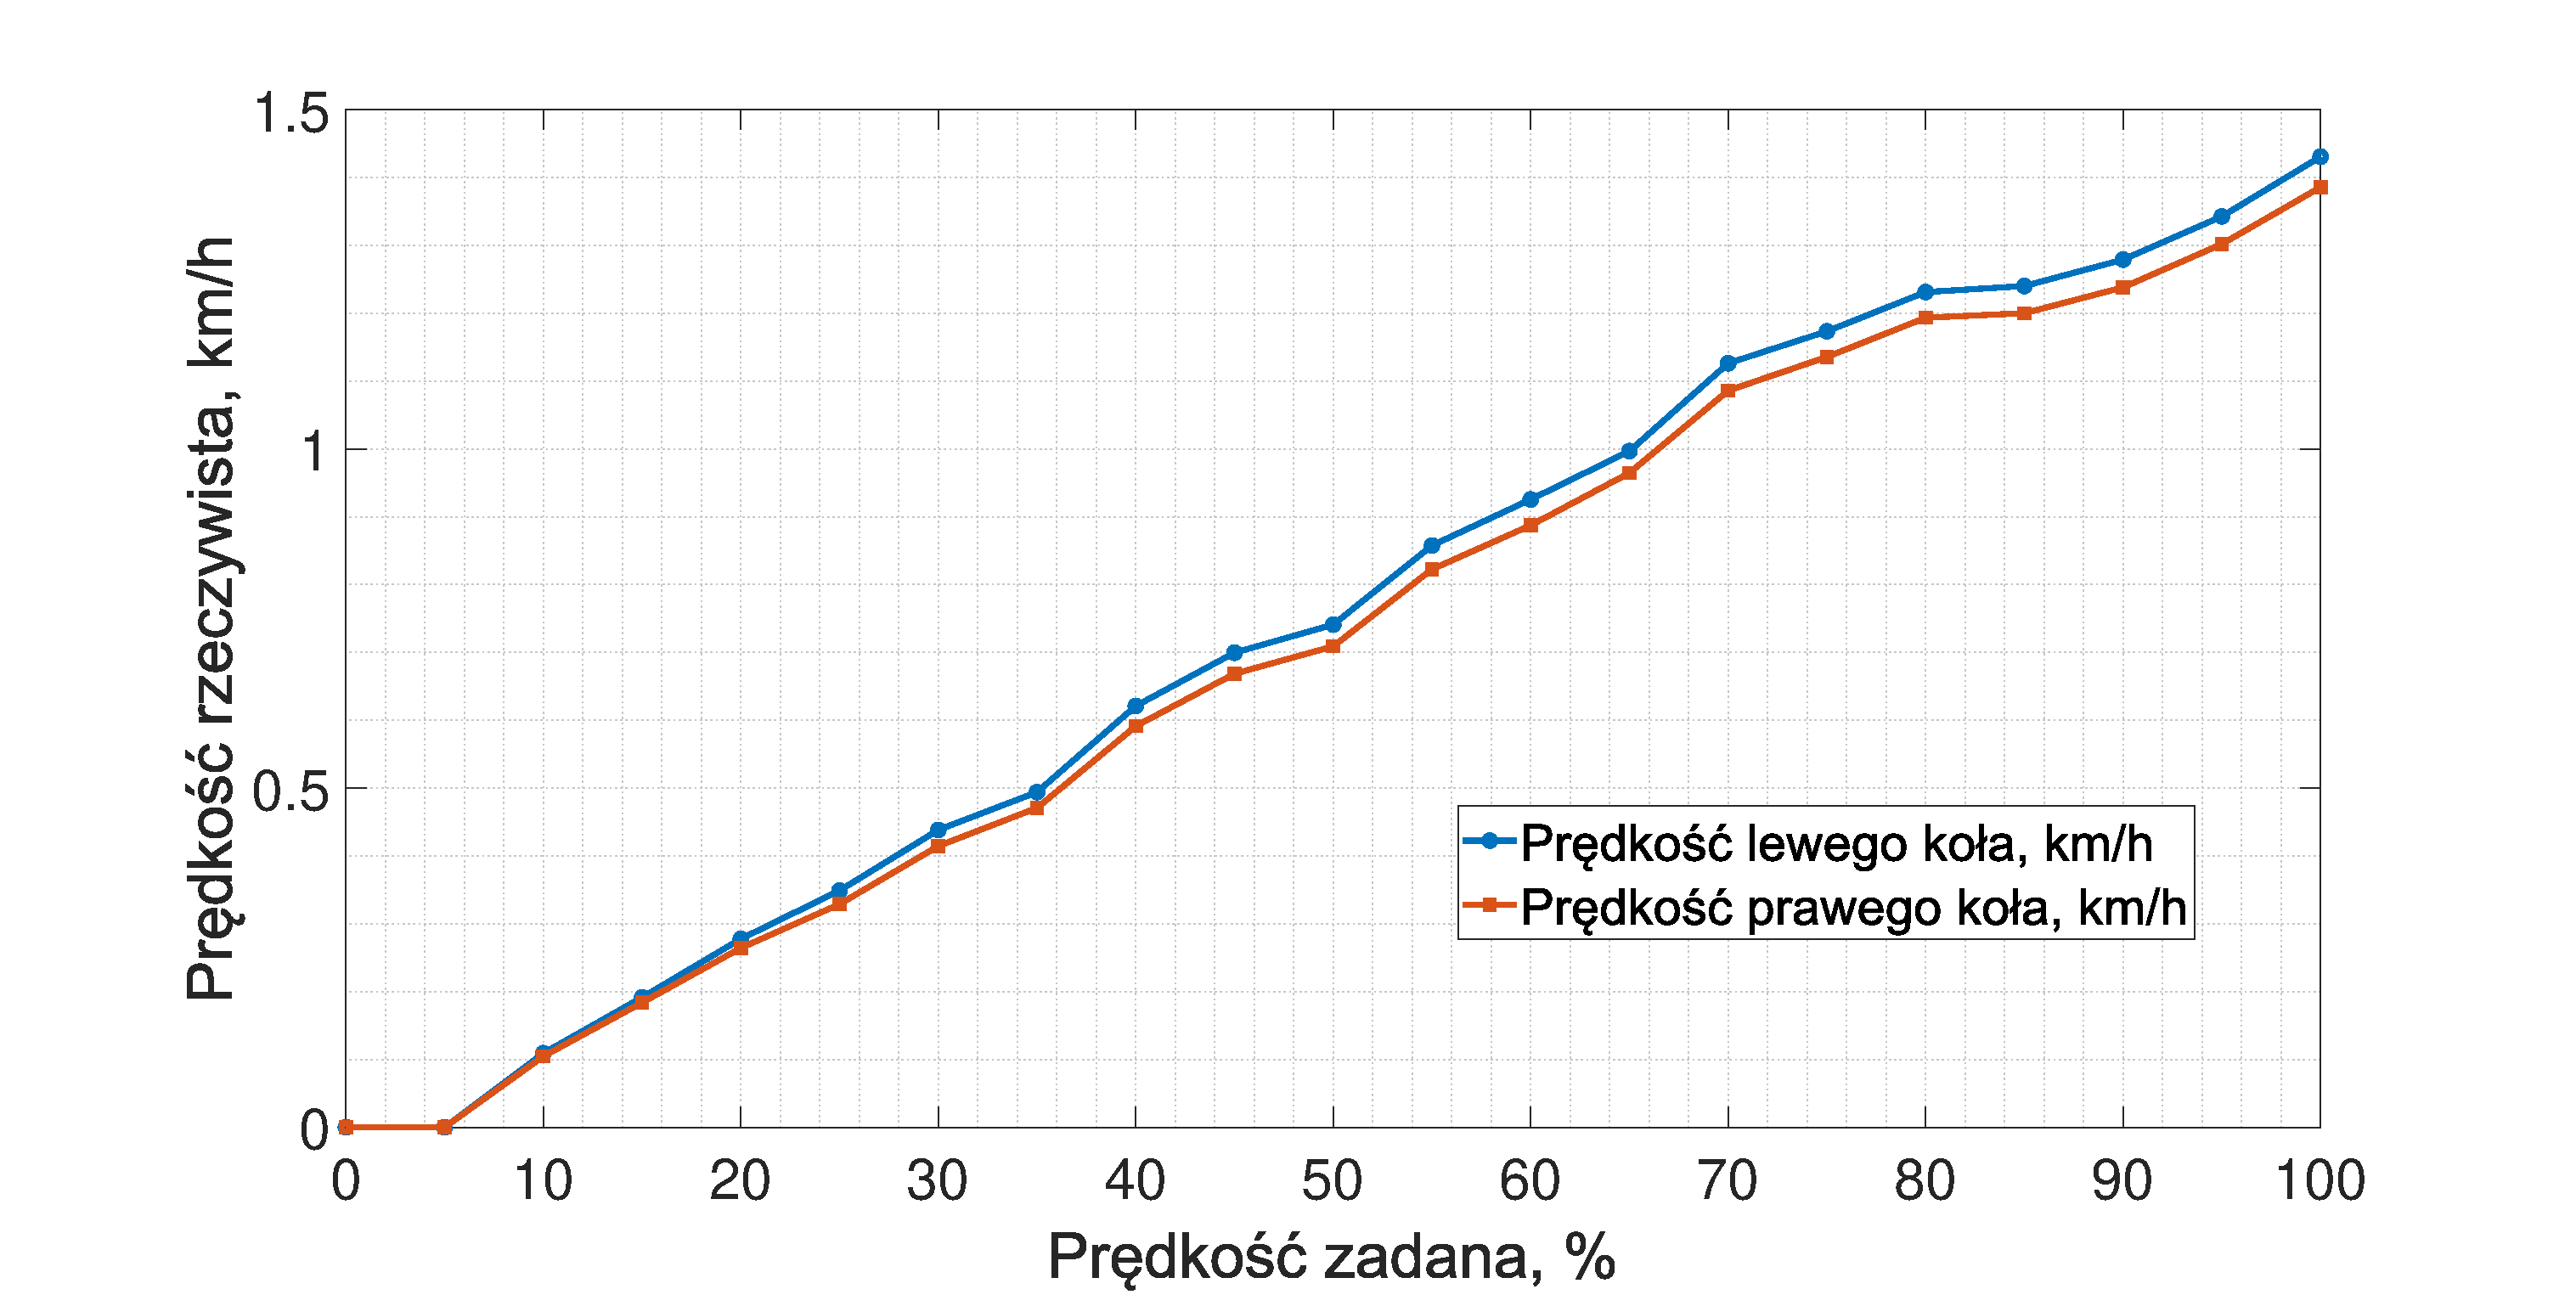
\includegraphics[scale=0.31]{images/charStat.eps}
    \captionof{figure}{Charakterystyki statyczne silników}
    \label{fig:charstatjalowy}
\end{center}
\vspace*{-1cm}

\section{Strojenie regulatorów PID prowadzącego i śledzącego}
By ograniczyć ilość wykresów, których osobno byłoby kilkadziesiąt stron, kolejne iteracje zmiany tego samego parametru umieszczono na wspólnych wykresach. Strojenie odbywa się metodą doświadczalną.
\vspace*{-0.5cm}

\subsection*{Wzmocnienia proporcjonalne regulatora prowadzącego i~śledzącego}
Na Rysunku \ref{fig:strojeniekp} przedstawiono strojenie parametru K\textsubscript{P}.
\vspace*{-1cm}

\begin{center}
    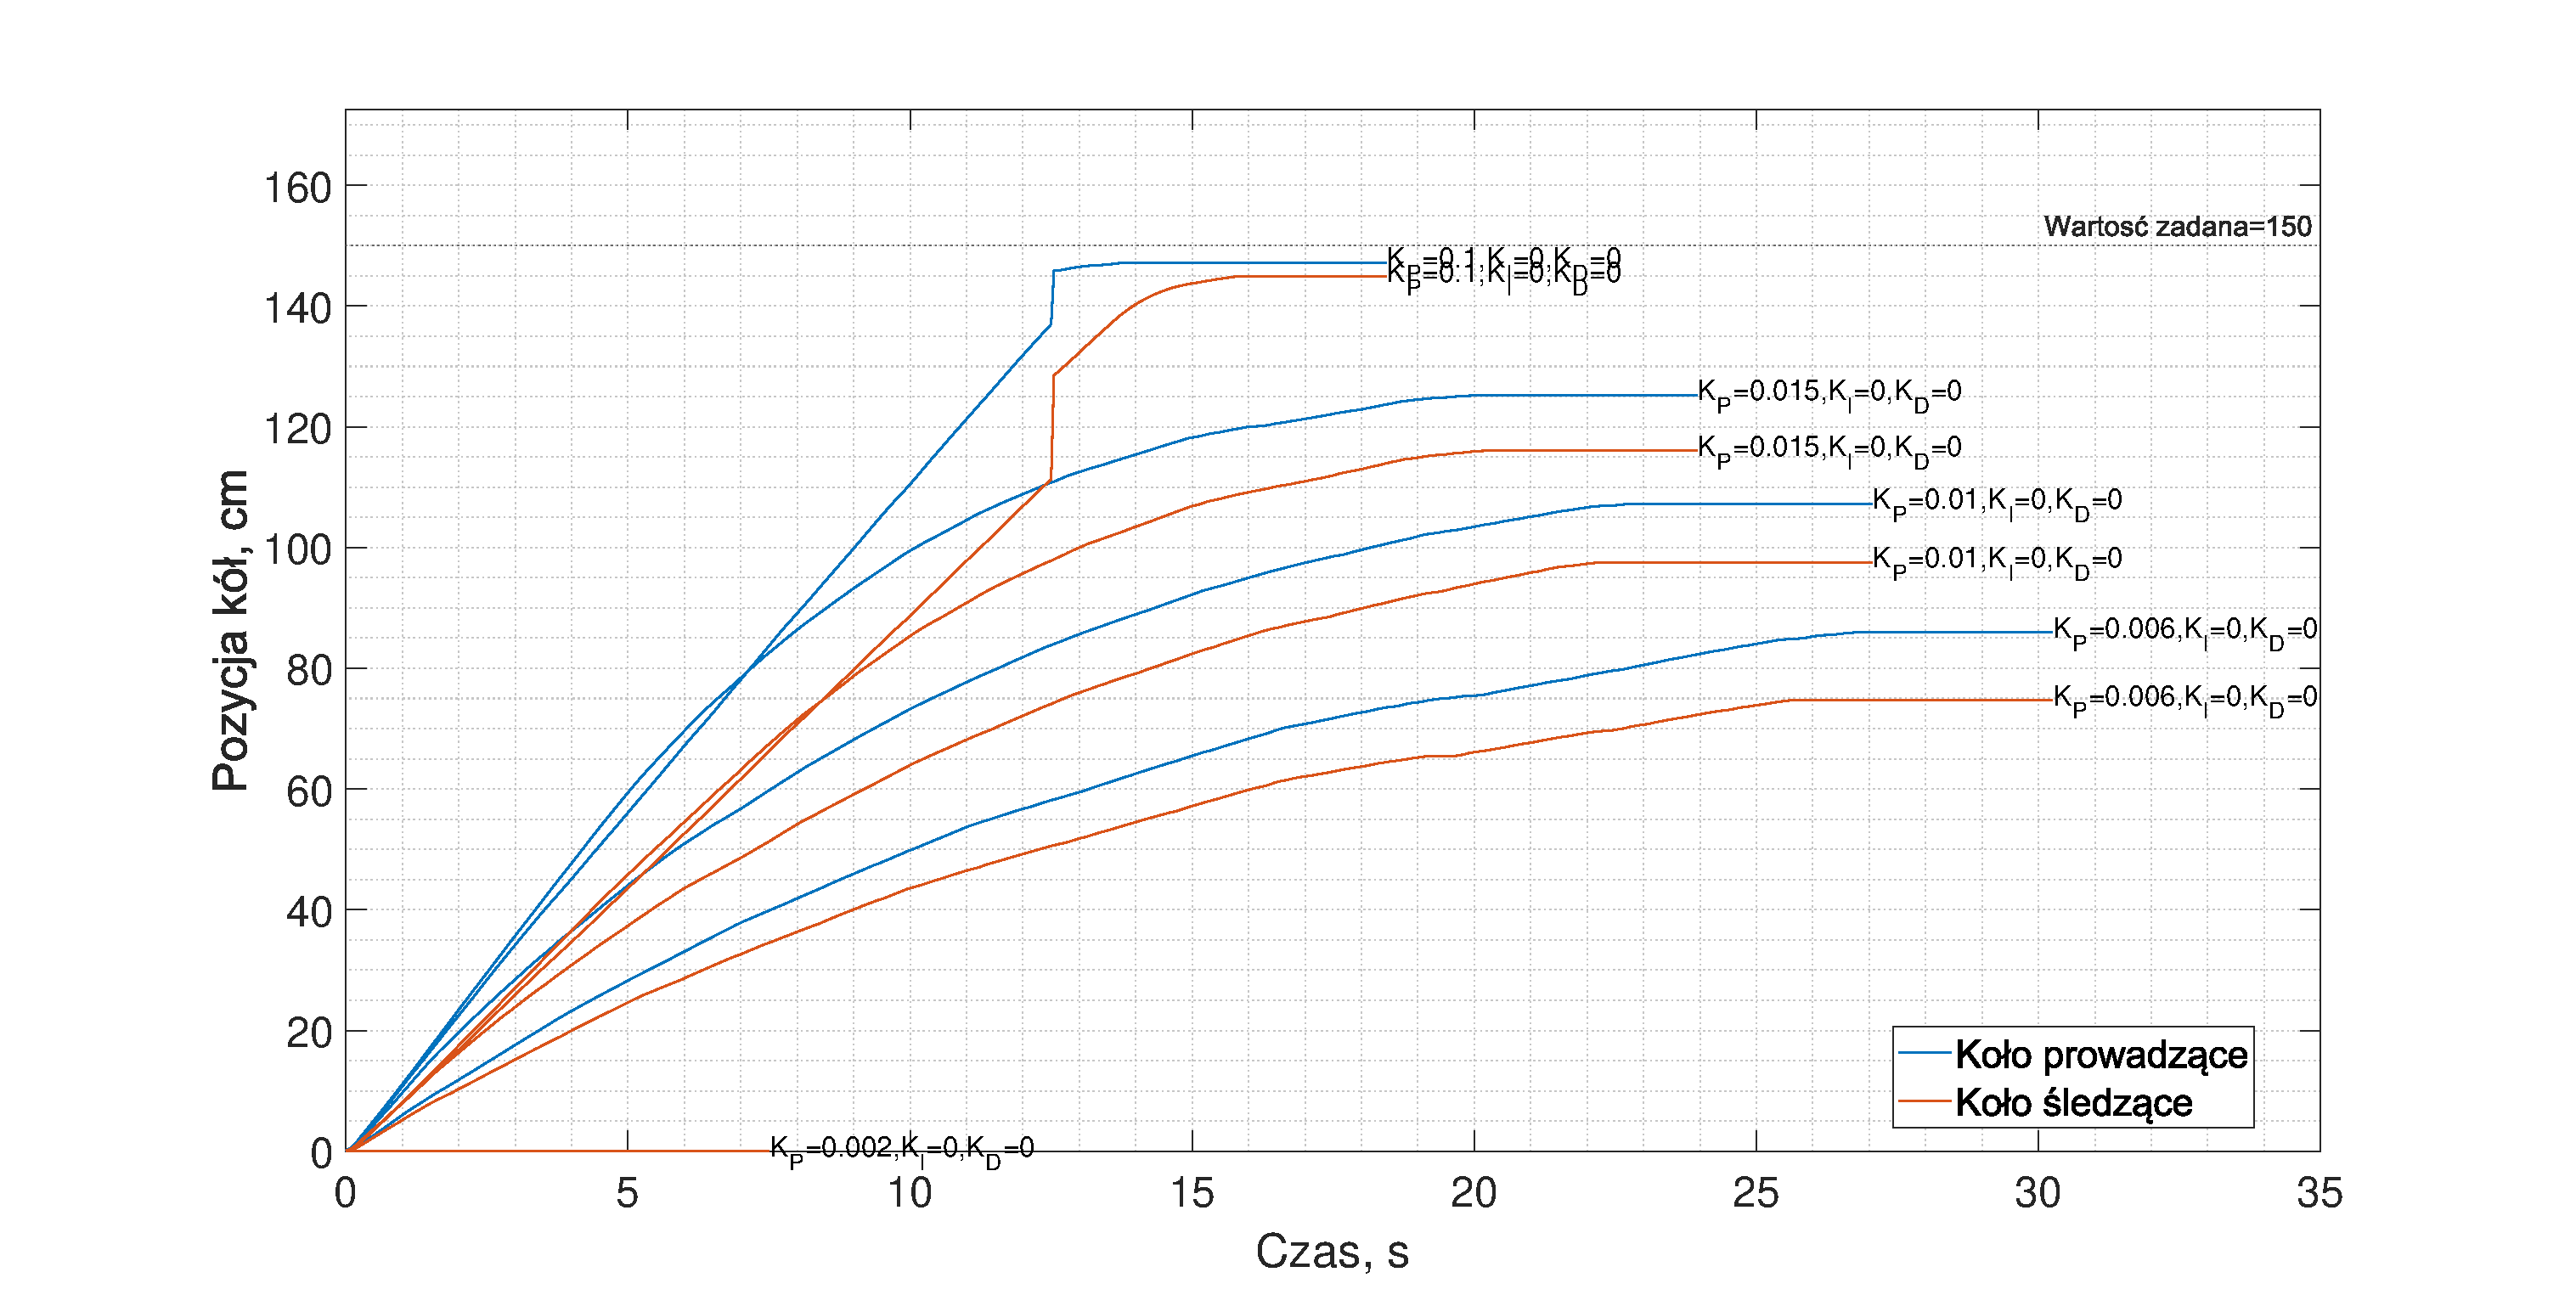
\includegraphics[scale=0.32]{images/strojenieKp.eps}
    \captionof{figure}{Porównanie odpowiedzi układu na zmianę parametru K\textsubscript{P}}
    \label{fig:strojeniekp}
\end{center}

Widoczne jest, że wzmocnienie K\textsubscript{P}=0.002 jest zbyt małe, by pojazd ruszył z~miejsca (nie pokonuje oporu statycznego). Potrzebne jest wzmocnienie znajdujące się gdzieś w~przedziale K\textsubscript{P}$\in \left(0.002;0.006\right)$. Dla K\textsubscript{P}=0.1 uchyb jest bardzo mały, nawet bez części całkującej. Widoczny jest nagły skok odpowiedzi dla K\textsubscript{P}=0.1 pomiędzy 12~a~13~sekundą, którego powód jest nieznany. Jedną z~hipotez jest utracenie przez koła przyczepności na ułamek sekundy, tym samym wpadając w~lekki poślizg i~zwiększając obroty. Możliwy jest również inny błąd pomiaru.

\subsection*{Dodanie członu całkującego regulatora prowadzącego i śledzącego}
Na Rysunku \ref{fig:strojenieki} przedstawiono zmianę odpowiedzi układu po dodaniu parametru K\textsubscript{I} i~jednoczesnej modyfikacji K\textsubscript{P}.
\begin{center}
    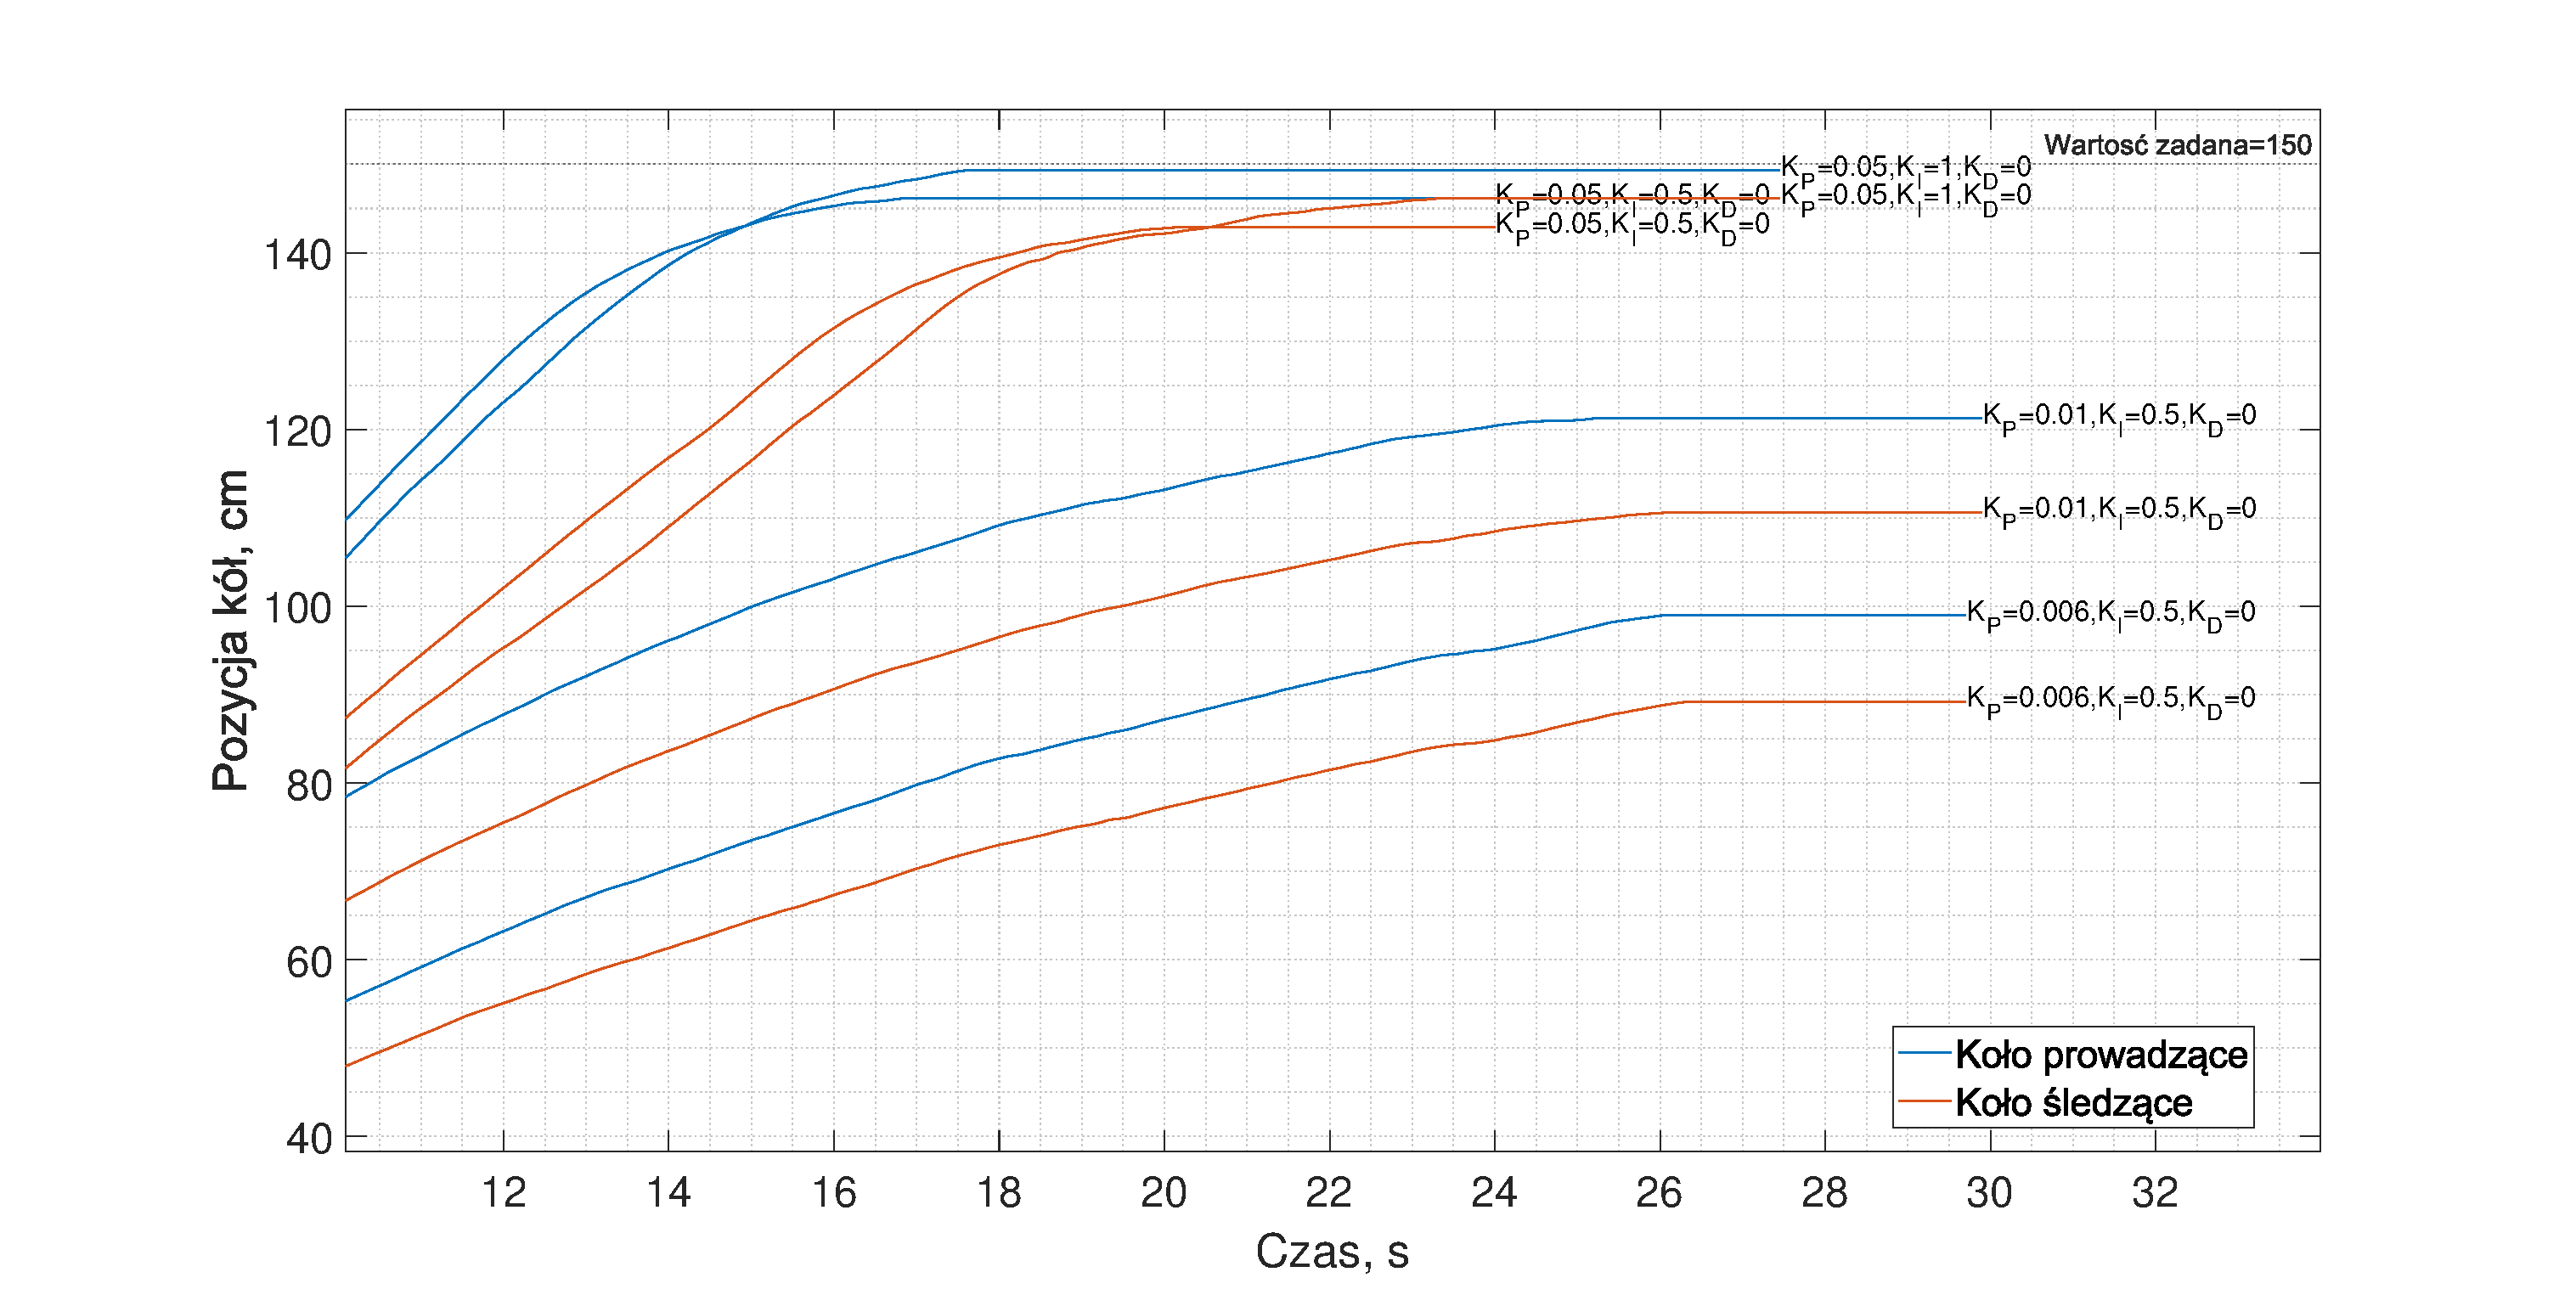
\includegraphics[scale=0.32]{images/strojenieKi.eps}
    \captionof{figure}{Porównanie odpowiedzi układu na zmianę parametrów K\textsubscript{P} i K\textsubscript{I}}
    \label{fig:strojenieki}
\end{center}

Jak widać, nawet dla K\textsubscript{P}=0.05 czyli mniejszego niż najlepsze uzyskane w~poprzednim kroku, używając wzmocnienia K\textsubscript{I}=1, uchyb koła prowadzącego zostaje zniwelowany do wartości bliskiej 0. Jako że koło śledzące jest tym, które w~następnym kroku zostanie zsynchronizowane z~prowadzącym, a~samo koło prowadzące daje dobrą odpowiedź na aktualne parametry nie oscylując przy tym, wzmocnienie K\textsubscript{D} pozostanie wyzerowane, tym samym nie dodając do sygnału części różniczkującej regulatora.~W dalszych krokach używane będą parametry regulatorów K\textsubscript{P}=0.05, K\textsubscript{I}=1, oraz K\textsubscript{D}=0.

\section{Strojenie regulatora PID synchronizującego}
